\chapter{Results}
\label{chp:results}

UNINETT has provided NetFlow data over December 2013, in the NetFlow file format.
To simplify implementation, \gls{nfdump} was used to convert the flows to \gls{csv} files.
SpreadRank was run on the flows logged by one router over one day, one week, two weeks and one month.
Calculation of SpreadRank scores only took some minutes to complete,
 but the conversion to \gls{csv} took a few hours to complete.
This was likely due to the fact that \gls{nfdump} had to read the compressed NetFlow files from \gls{HDFS},
 and then write uncompressed \gls{csv} files onto the same HDFS volume.

After calculation, \gls{Giraph} writes output files containing all vertex IDs as values.
The vertex value (figure~\ref{fig:datatype-spreadrank-vertex-value}) consists of the depth and the spreading of the vertex.
A Giraph OutputFormat was implemented in order to make the output files better parseable using GNU utilities.

\section{Longest path}
Most \gls{service}s on the internet do not exhibit spreading.
Figure~\ref{fig:spreading-perstep-pie} shows a plot of spreading per vertex, calculated over NetFlow information from one router during one day and during one month.
Most vertices have a spreading of zero, one or two.
A spreading of zero typically indicates a server, one typically indicates a client (its traffic reaches to the servers) and a spreading of two often indicates a hybrid, but it can also indicate a simple proxy server.
Higher spreading indicates end-hosts that do participate in spreading.
This is typical for DNS servers, SMTP servers and BGP routers.

\begin{figure}[h!]
	\caption{Spreading per vertex}
	\label{fig:spreading-perstep-pie}
	\centering
		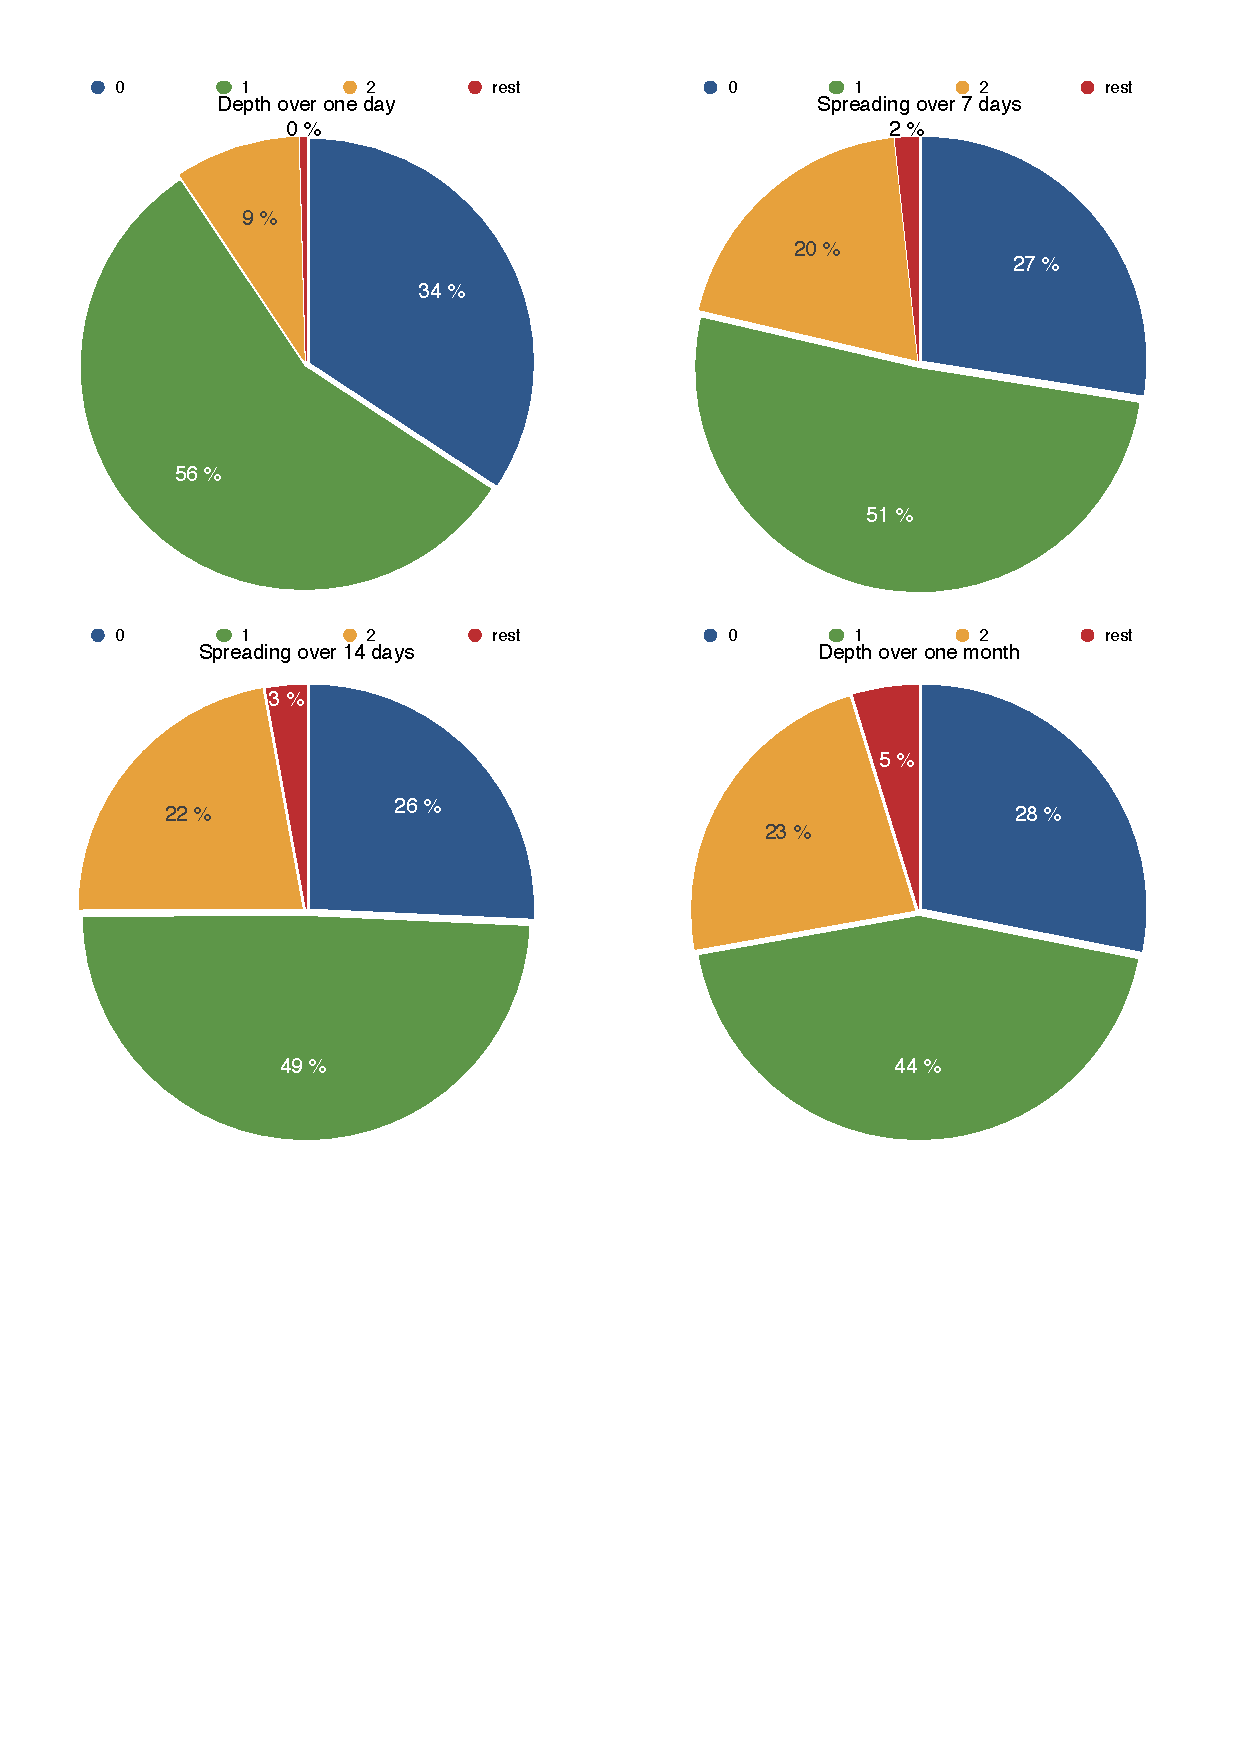
\includegraphics[width=1\textwidth]{spreading-perstep-pie}
\end{figure}

\section{Protocols}
After filtering traffic such that only \gls{service}s with a spreading of one or higher,
 and a depth of two or higher remain, only a few protocols remain (figure~\ref{fig:protocol-pie}).
This confirms the assumptions stated in section~\ref{sec:depth} and chapter~\ref{chp:anomalies},
 which is that spreading is expected to happen only on certain protocols.
\Gls{BGP}, \gls{DNS} and \gls{SMTP} are expected to spread, due to the way the protocols work.
\Gls{BGP} is used between routers to calculate shortest paths; routers need to keep each other updated and thus all will eventually initiate a connection,
 which might lead to another router relaying the information to other routers.
\gls{DNS} and \gls{SMTP} are both protocols where clients send their request to a server that is close to them,
 and the server will then handle the request.
In the case of \gls{DNS}, this means that the server will answer with information from its cache, or look the requested record up itself.
In the case of \gls{SMTP}, this means that the server will forward e-mail to the mail server of the recipient.
These services yield high depths, as virtually any server providing these services can forward information it receives.


\begin{figure}[h!]
	\caption{Distribution of protocols that exhibit spreading}
	\label{fig:protocol-pie}
	\centering
		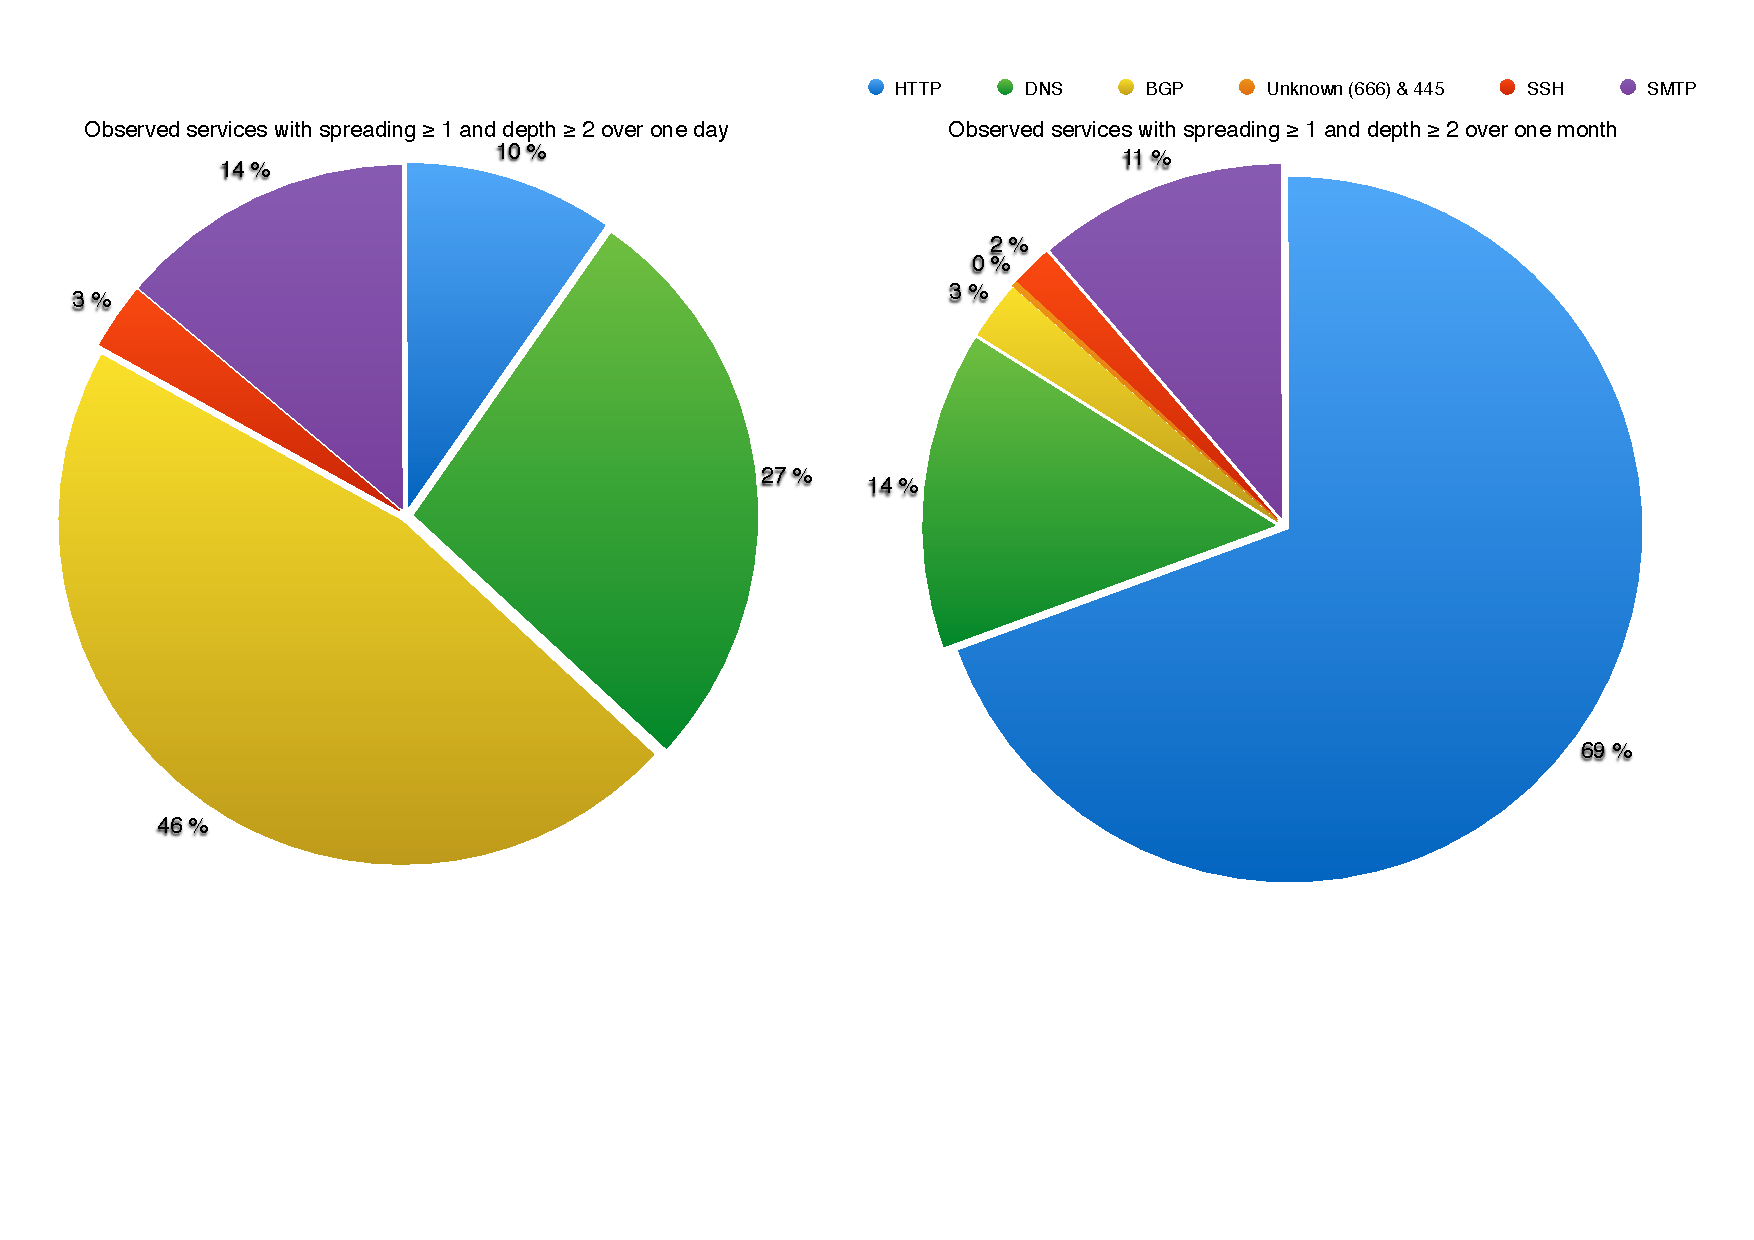
\includegraphics[width=1\textwidth]{protocol-pie}
\end{figure}


The \gls{SSH} and \gls{HTTP} protocols also show up with higher spreading.
This may be due to home servers often serving web pages,
 and Linux-based home servers will typically also listen for SSH for remote management.
HTTP spreading is discussed in more detail in section~\ref{sec:http}.

Remarkable results are spreading on ports 666 and 445.
Port 666 is officially allocated as the port for computer game Doom~\cite{rfc1700},
 but in practice it is also used by viruses.
Only one instance of spreading over port 666 was observed over one month.
Port 445 is used by Microsoft Windows for sharing files, but it is also abused for denial of service attacks~\cite{lazarevic2003comparative}.
Because of this, it is unknown whether this spreading was due to an attack, or simply some users that had used Microsoft Windows File Sharing.

\section{Plot}
Individual observed services with a reach of one or higher are plotted in figure~\ref{fig:31day}.
It is based on one month worth of NetFlow.

\begin{itemize}
\item The X axis shows \gls{spreading} -- the amount of end-hosts reached via spreading -- the amount of messages received in total.
\item The Y axis shows \gls{depth} -- the longest path.
\item The size of the dot shows the amount of observed \gls{client}s -- the amount of incoming connections to the end-host.
\end{itemize}

\begin{figure}[h!]
	\caption{End-hosts scored with SpreadRank over one month}
	\label{fig:31day}
	\centering
		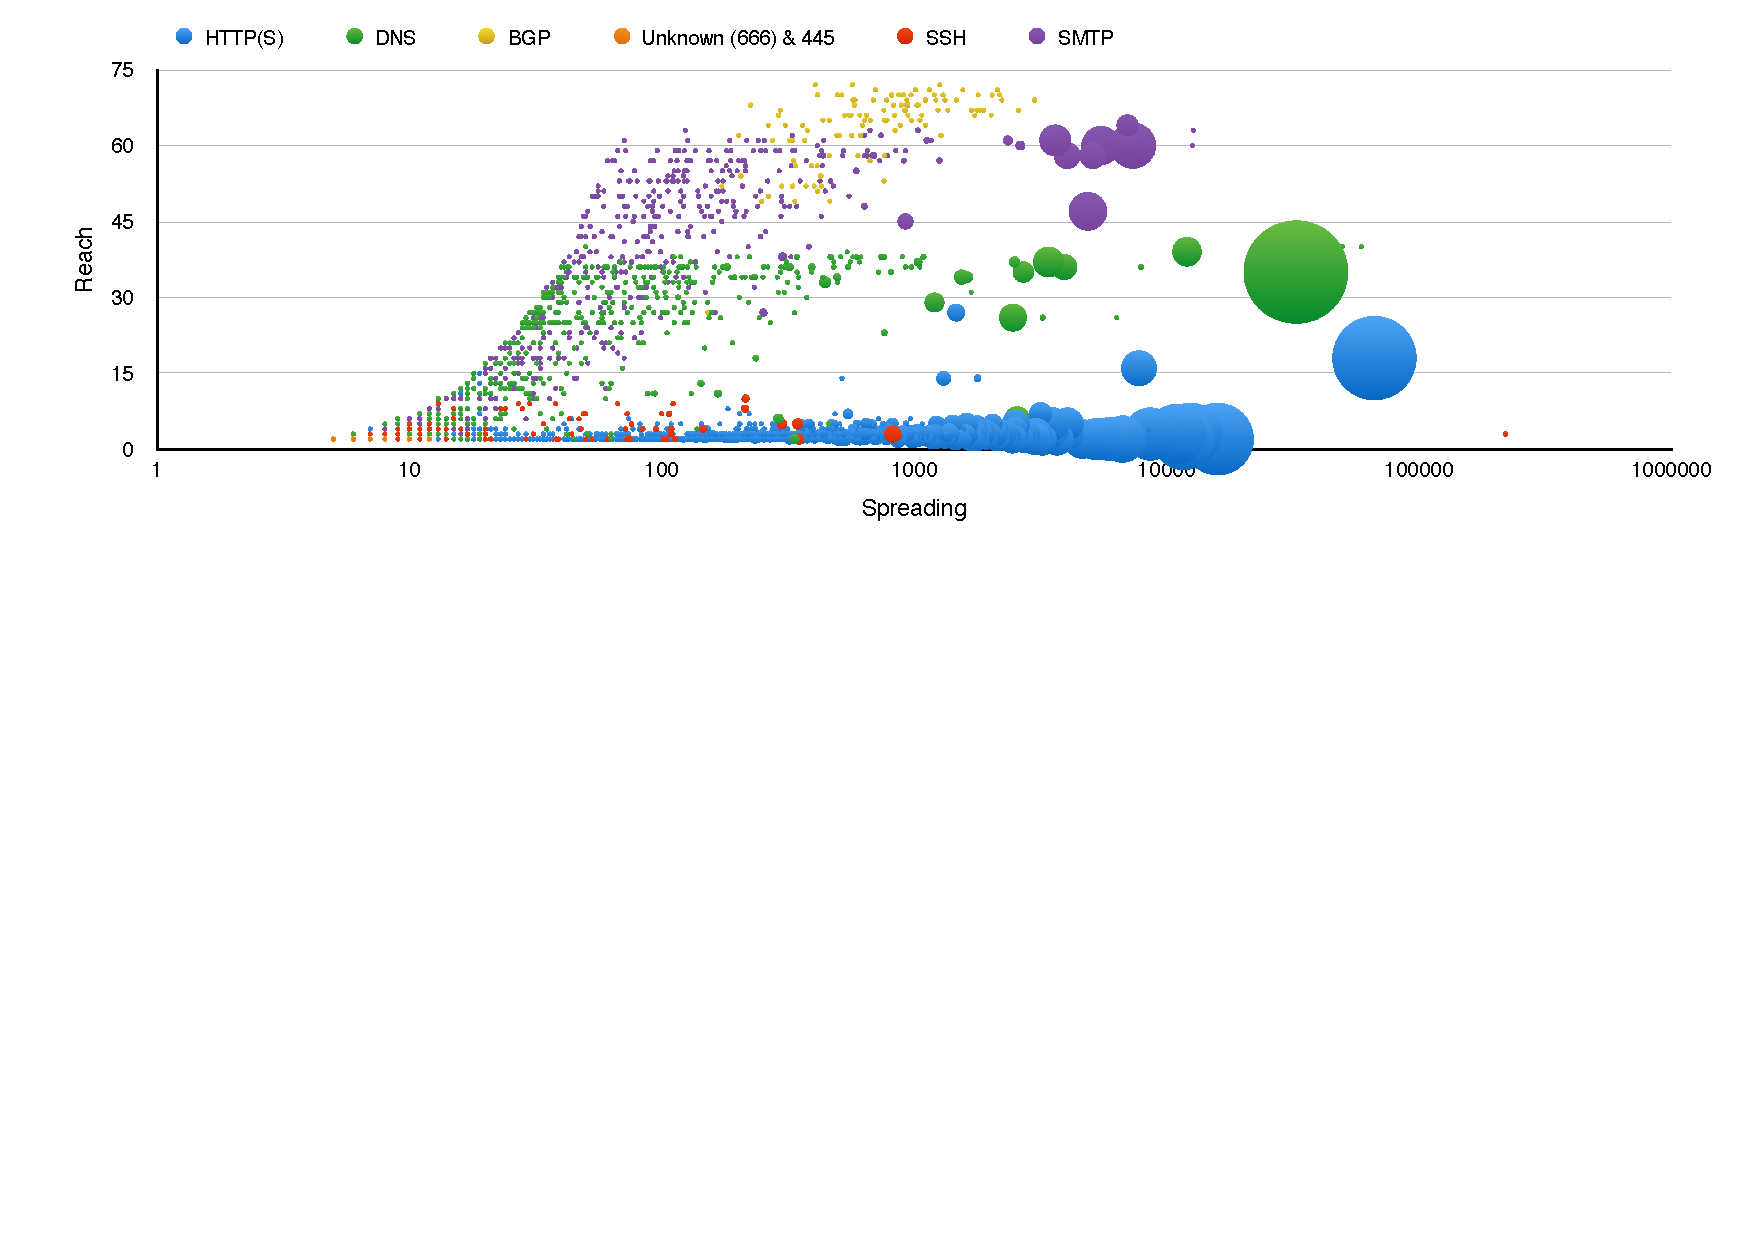
\includegraphics[width=1\textwidth]{31day}
\end{figure}

%The plots show a clear pattern.
%The pattern is not very clear in the plot from one day, but becomes clearer in the subsequet plots.
%The curve on the left side is simply an effect of the logarithmic scale of the plot;
% spreading can not be lower than the depth.
%The plot has an E shape, with many services with few clients at the low end of the spreading,
% and few services with many clients at the high end of the spreading.
%Each protocol in the plot has its maximum reach.
%The maximum reach is favoured by services with a high spreading, hence the E shape of the plot.

\section{Observed anomalies}
Figure~\ref{fig:31day} shows all observed IP-address + port number combinations with a depth of 2 or higher.
The best way to observe anomalies in this plot, is by Multi-class Anomaly Detection.
Multi-class classification assumes that the data set contains different distinct types of data~\cite{Chandola:2009:ADS:1541880.1541882}.
In the case of SpreadRank, these types of data are the port numbers.
Different ports are indicated with different colours in the plot, and it is apparent that there is a pattern.
It is also apparent that there are some outliers (figure~\ref{fig:spreadrank-pattern}, but there is no clear border between normal observations and anomalous observations.
However, a simple visual observation of the plot does give some interesting results.

\begin{figure}[h!]
	\caption{SpreadRank pattern over one month}
	\label{fig:spreadrank-pattern}
	\centering
		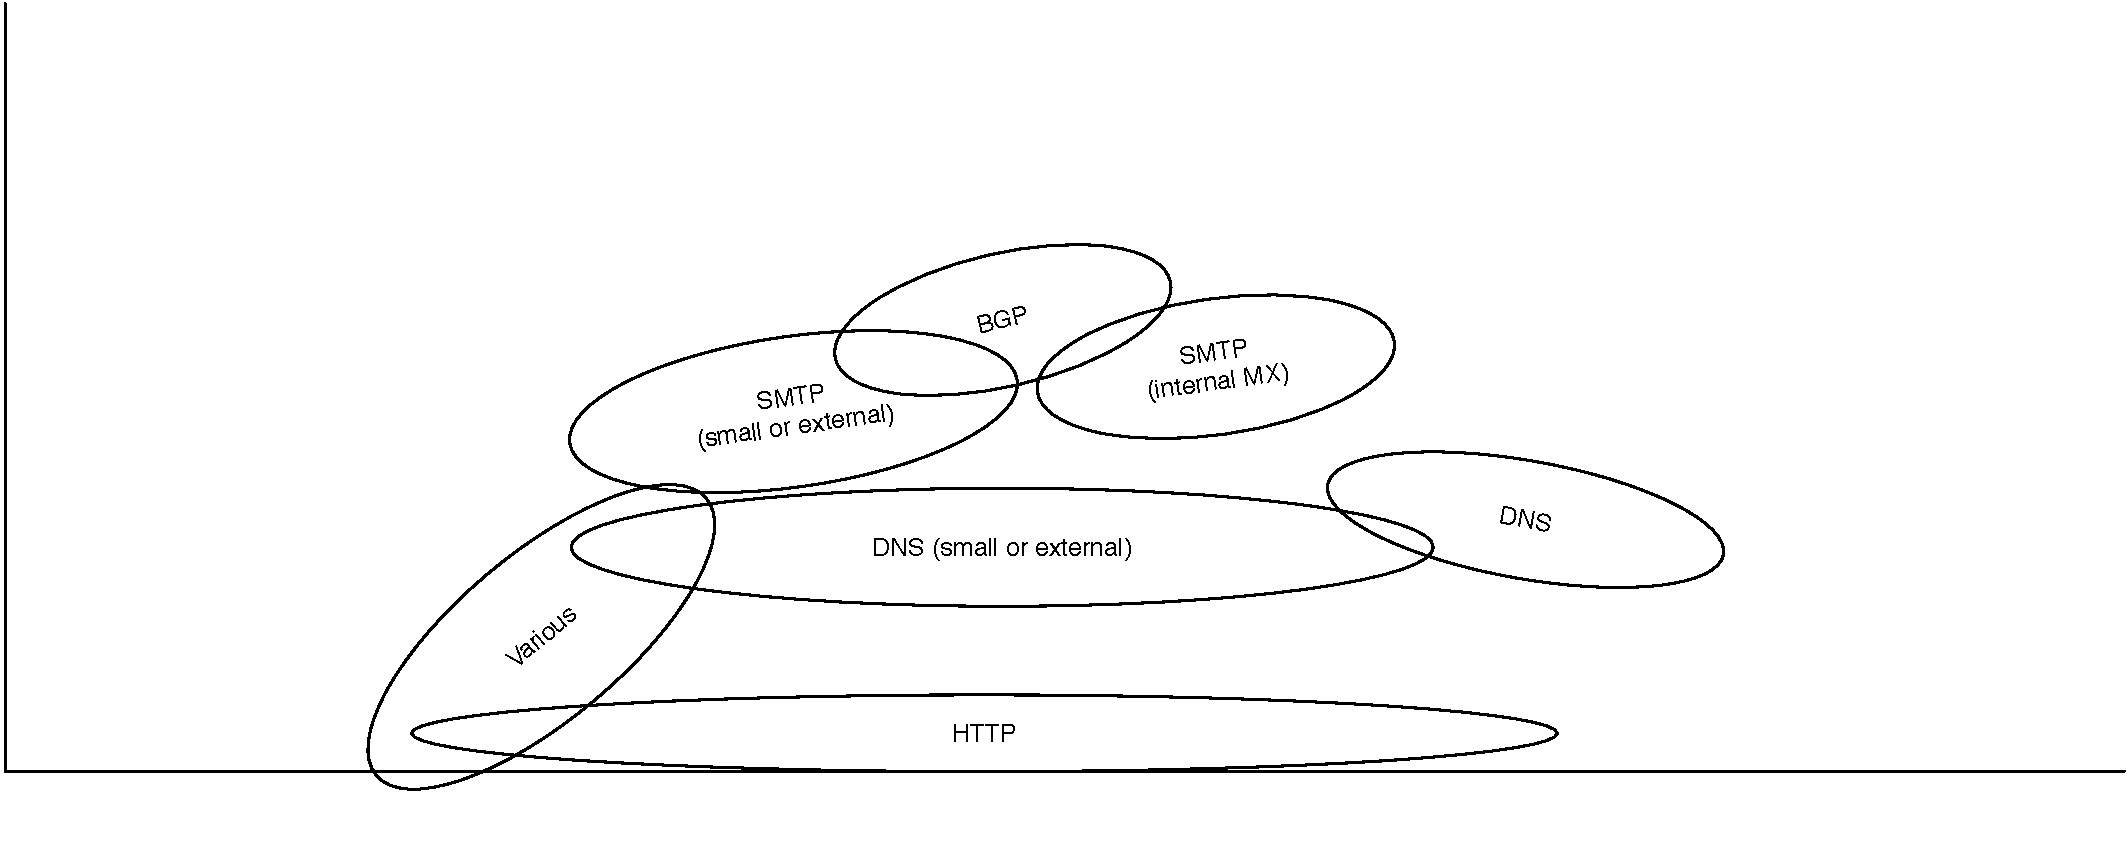
\includegraphics[width=1\textwidth]{spreadrank-pattern}
\end{figure}

\subsection{Botnet}
\label{ssec:botnet}

\begin{figure}[h!]
	\caption{HTTP and SSH traffic in SpreadRank over one month}
	\label{fig:31day-botnet}
	\centering
		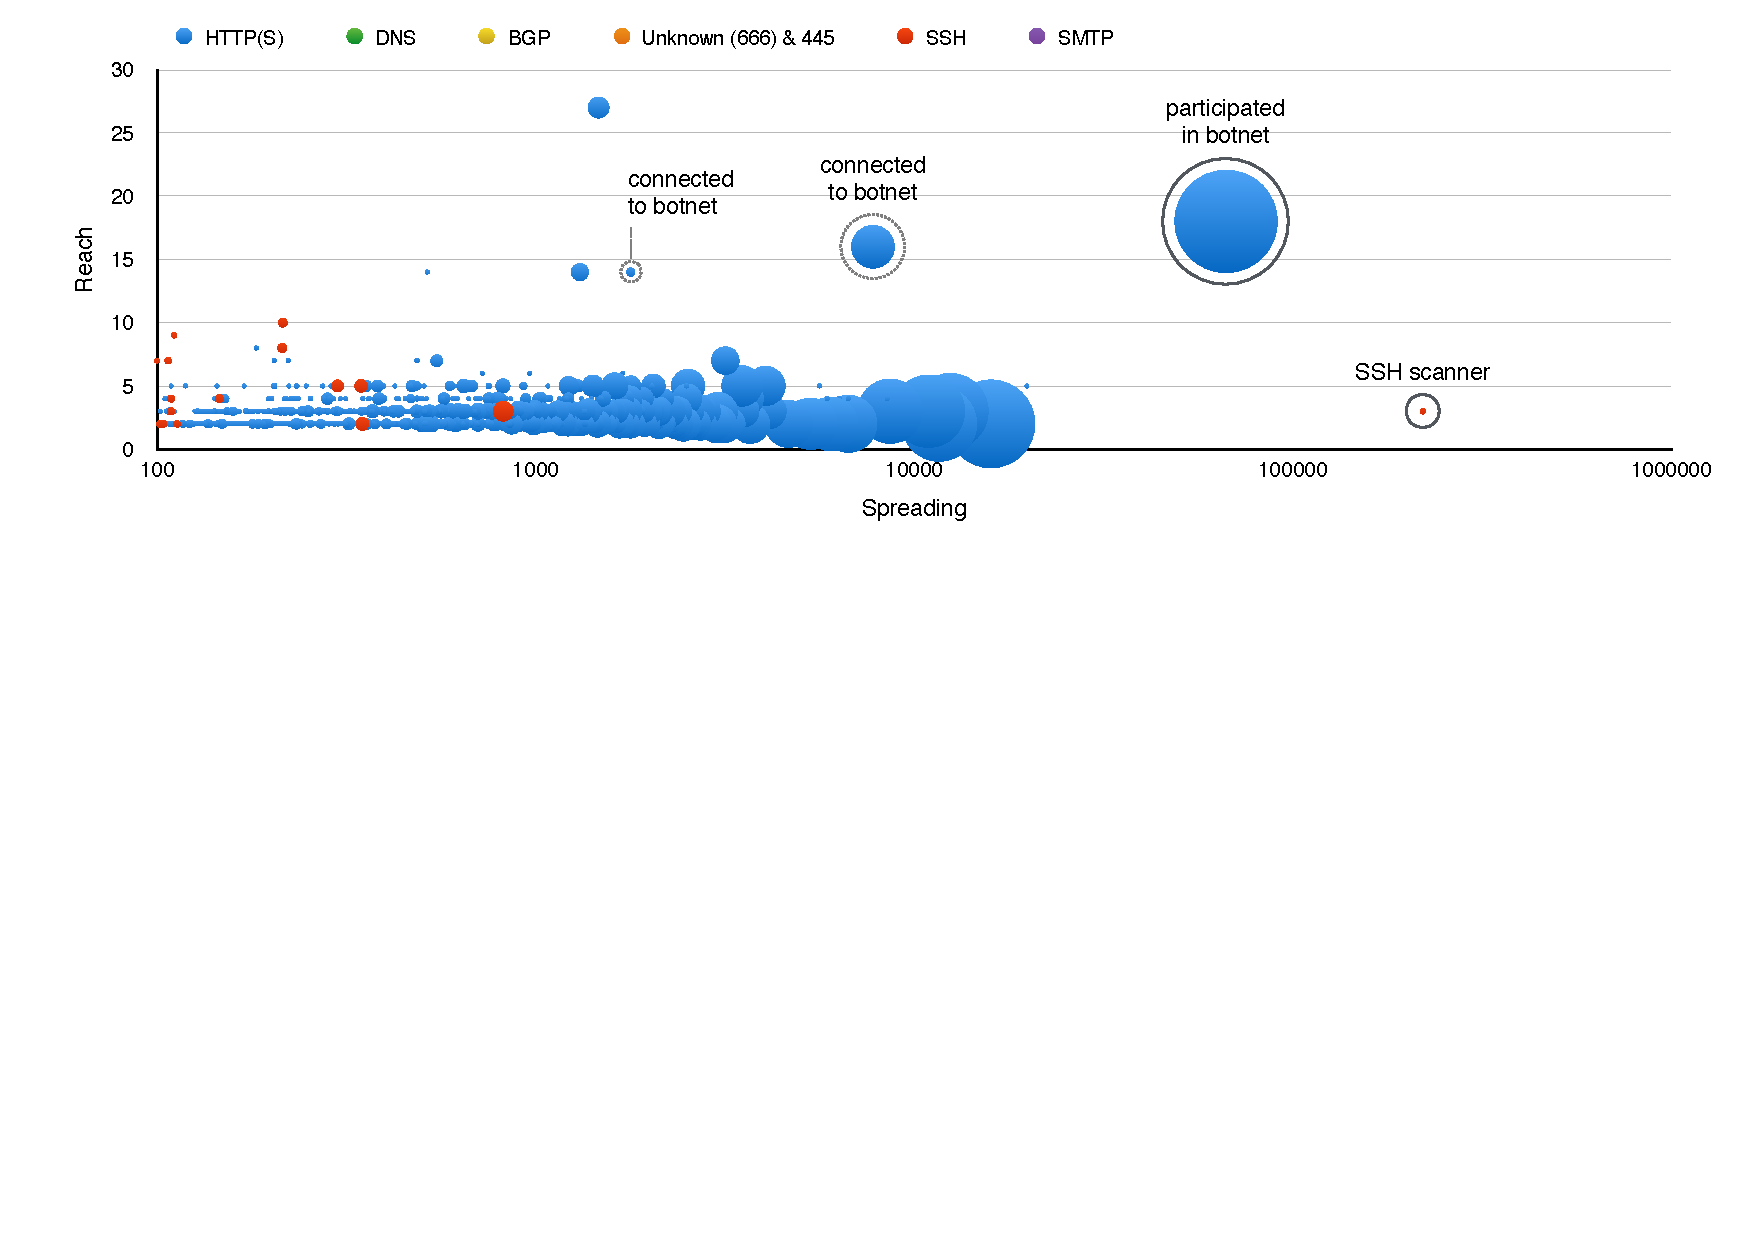
\includegraphics[width=1\textwidth]{31day-botnet}
\end{figure}

Figure~\ref{fig:31day-botnet} shows \gls{HTTP} and \gls{SSH} services.
Dots marked with a solid line are linked to hosts that were reported to CERT.
The tiny red SSH node at the right hand side has been involved in \gls{SSH} scanning,
 where it connects to many IP addresses in the hope to find an SSH server with a password it can guess.
The large HTTP node at the right hand side was confirmed participating in a botnet during December 2013,
 but it was not discovered until January.
The host had many incoming and outgoing connections over port 80 in December, but at the moment of writing the host was down (no response).
After analysing the logs with more detail, it appeared that it was contacted very often by servers hosting questionable content.
These servers were contacted by various clients at the \gls{ntnu} at a regular interval,
 but starting the 24th of December, some of these servers started contacting the machine at \gls{ntnu}.
On January 1st, 2014, UNINETT CERT received a report stating that the machine participated in a botnet.

By matching the IP addresses this botnet host had contact with,
 two additional hosts were discovered participating in the botnet.
These two hosts were not reported to CERT, and were therefore never investigated.
Since none of the machines are up at the moment of writing this thesis,
 no further investigation is done.

According to information from \gls{DNS}, the host that got reported to CERT is a machine at a faculty at \gls{ntnu}.
The two hosts that were found using SpreadRank are computers at two different student villages at \gls{ntnu}.
More precise information is available at UNINETT at the time of writing, but cannot be published in this thesis for privacy reasons.

\subsection{DNS}
\begin{figure}[h!]
	\caption{DNS traffic in SpreadRank over one month}
	\label{fig:31day-dns}
	\centering
		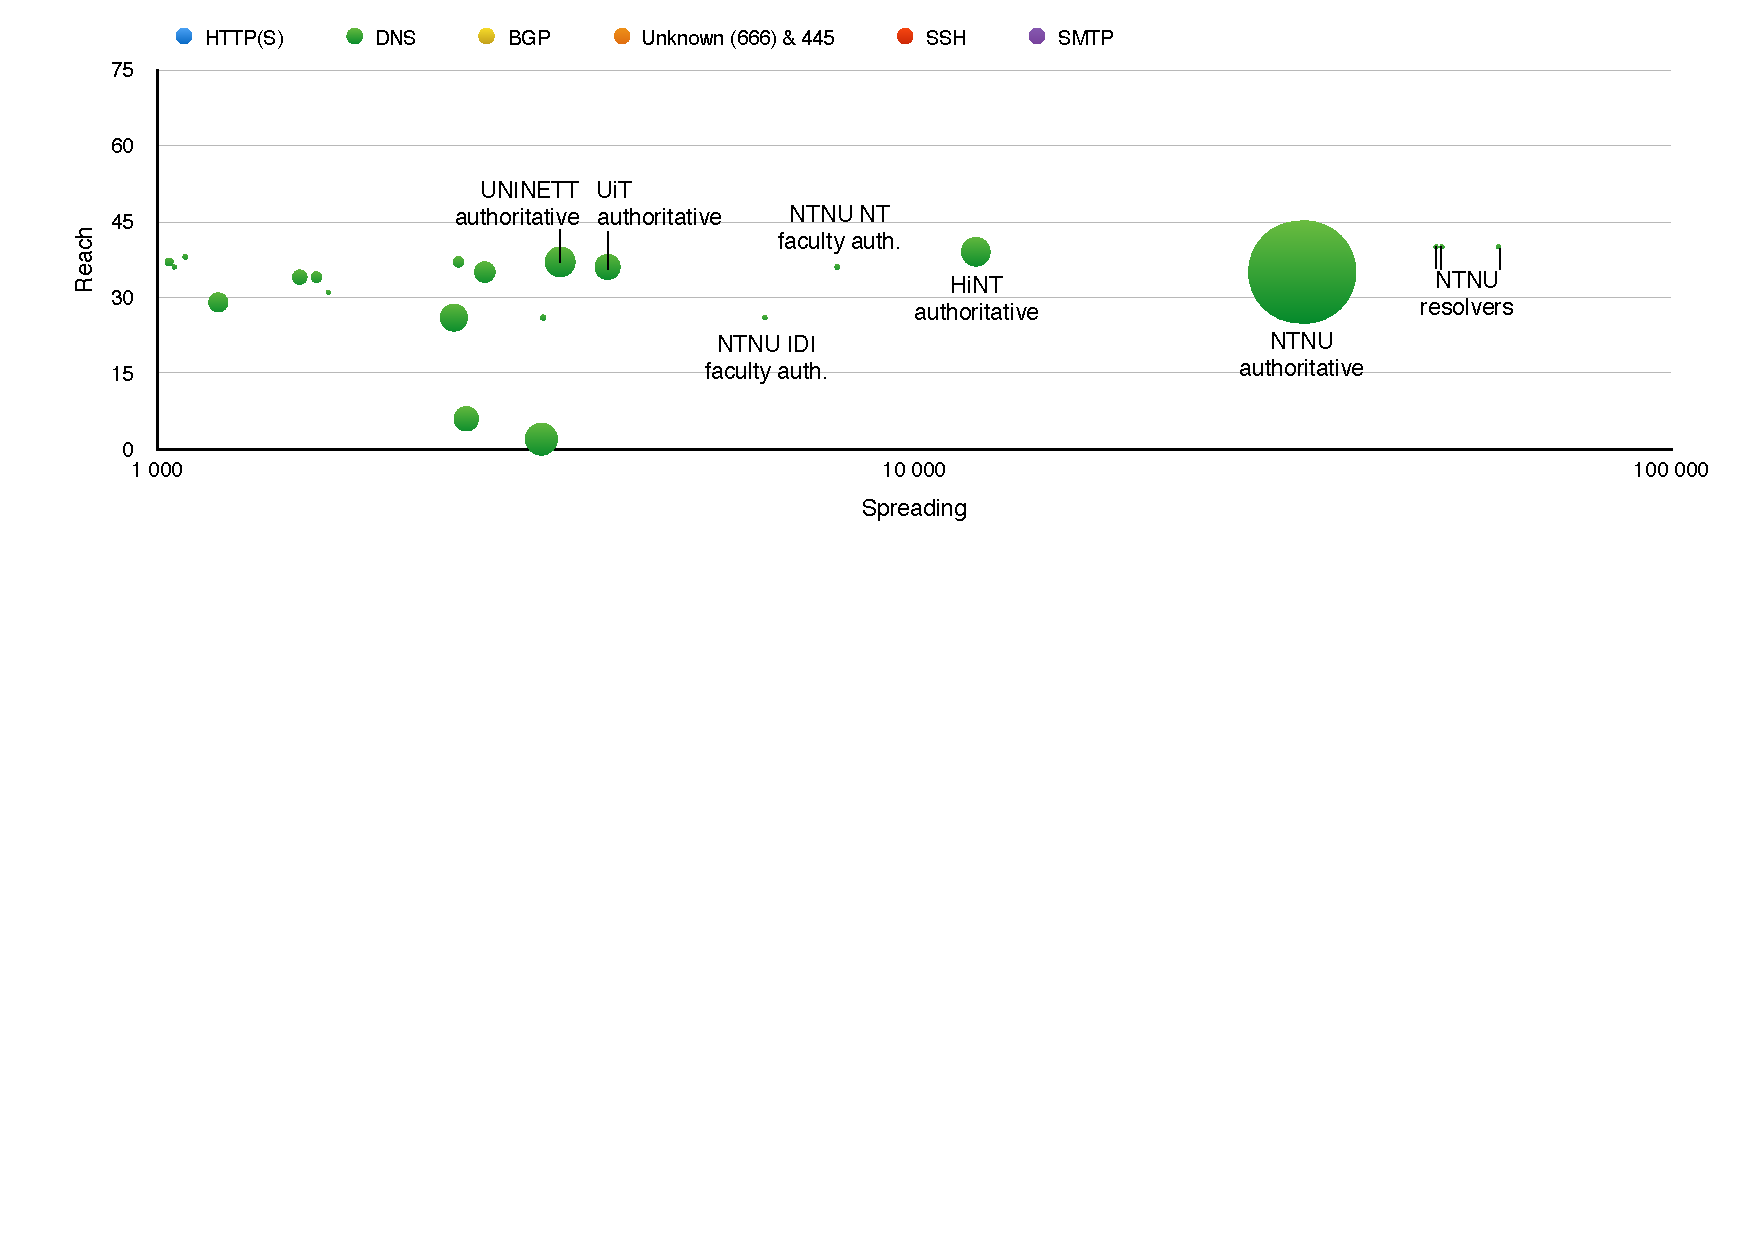
\includegraphics[width=1\textwidth]{31day-dns}
\end{figure}

Figure~\ref{fig:31day-dns} shows \gls{DNS} services, marked by which institution manages them.
DNS resolvers are used to lookup DNS records for hosts inside the network.
These resolvers cannot be used from the outside, which is why the dots are small;
 the clients are inside the institution, and are therefore not logged by UNINETT's core routers (figure~\ref{fig:nodes}).

Authoritative DNS servers that cause spreading may seem like an anomaly;
 Authoritative DNS servers answer queries from clients and do not send queries themselves.
However, there is an explanation for this spreading:
In order to keep DNS zones available, most domains use multiple DNS servers.
These DNS servers must keep in sync, and will therefore periodically contact a master server if it is not itself the master for the DNS zone.


\subsection{SMTP}
SMTP is the protocol used for mail delivery, where sometimes an e-mail is forwarded a couple of times before it reaches a mailbox.
This causes spreading, which can be seen in figure~\ref{fig:31day}.
There are some SMTP services that have very high spreading, but these are simply hosts that handle high amounts of mail per day.


\section{Performance}
UNINETT made a server cluster available for the analysis.
This cluster is installed with Apache Hadoop~\cite{Borthakur:2011:AHG:1989323.1989438}, and consists of 15 worker machines with 4~CPUs and 16~GB RAM each.
In addition, there are two HDFS name-nodes and one YARN manager, which have 4~CPUs, and 10~GB RAM each.

Figure~\ref{fig:performance} shows how SpreadRank performs on this cluster,
 by NetFlow logs over one day, one week, two weeks and one month.
The logs are cumulative, so the one week log also contains the information from the one day log, etc.
Since every task is devided over multiple workers, of which multiple can exist on one worker machine,
 the calculation times fluctuate.
The figure shows one measurement where SpreadRank is run four times, for different NetFlow log sizes.
An interesting result is that the calculation of one week takes slightly longer than the calculation of two weeks.
This is probably by accident, the job may have been scheduled in such a way that multiple workers were located on the same physical machine.

\begin{figure}[h!]
	\caption{Time used to calculate SpreadRank}
	\label{fig:performance}
	\centering
		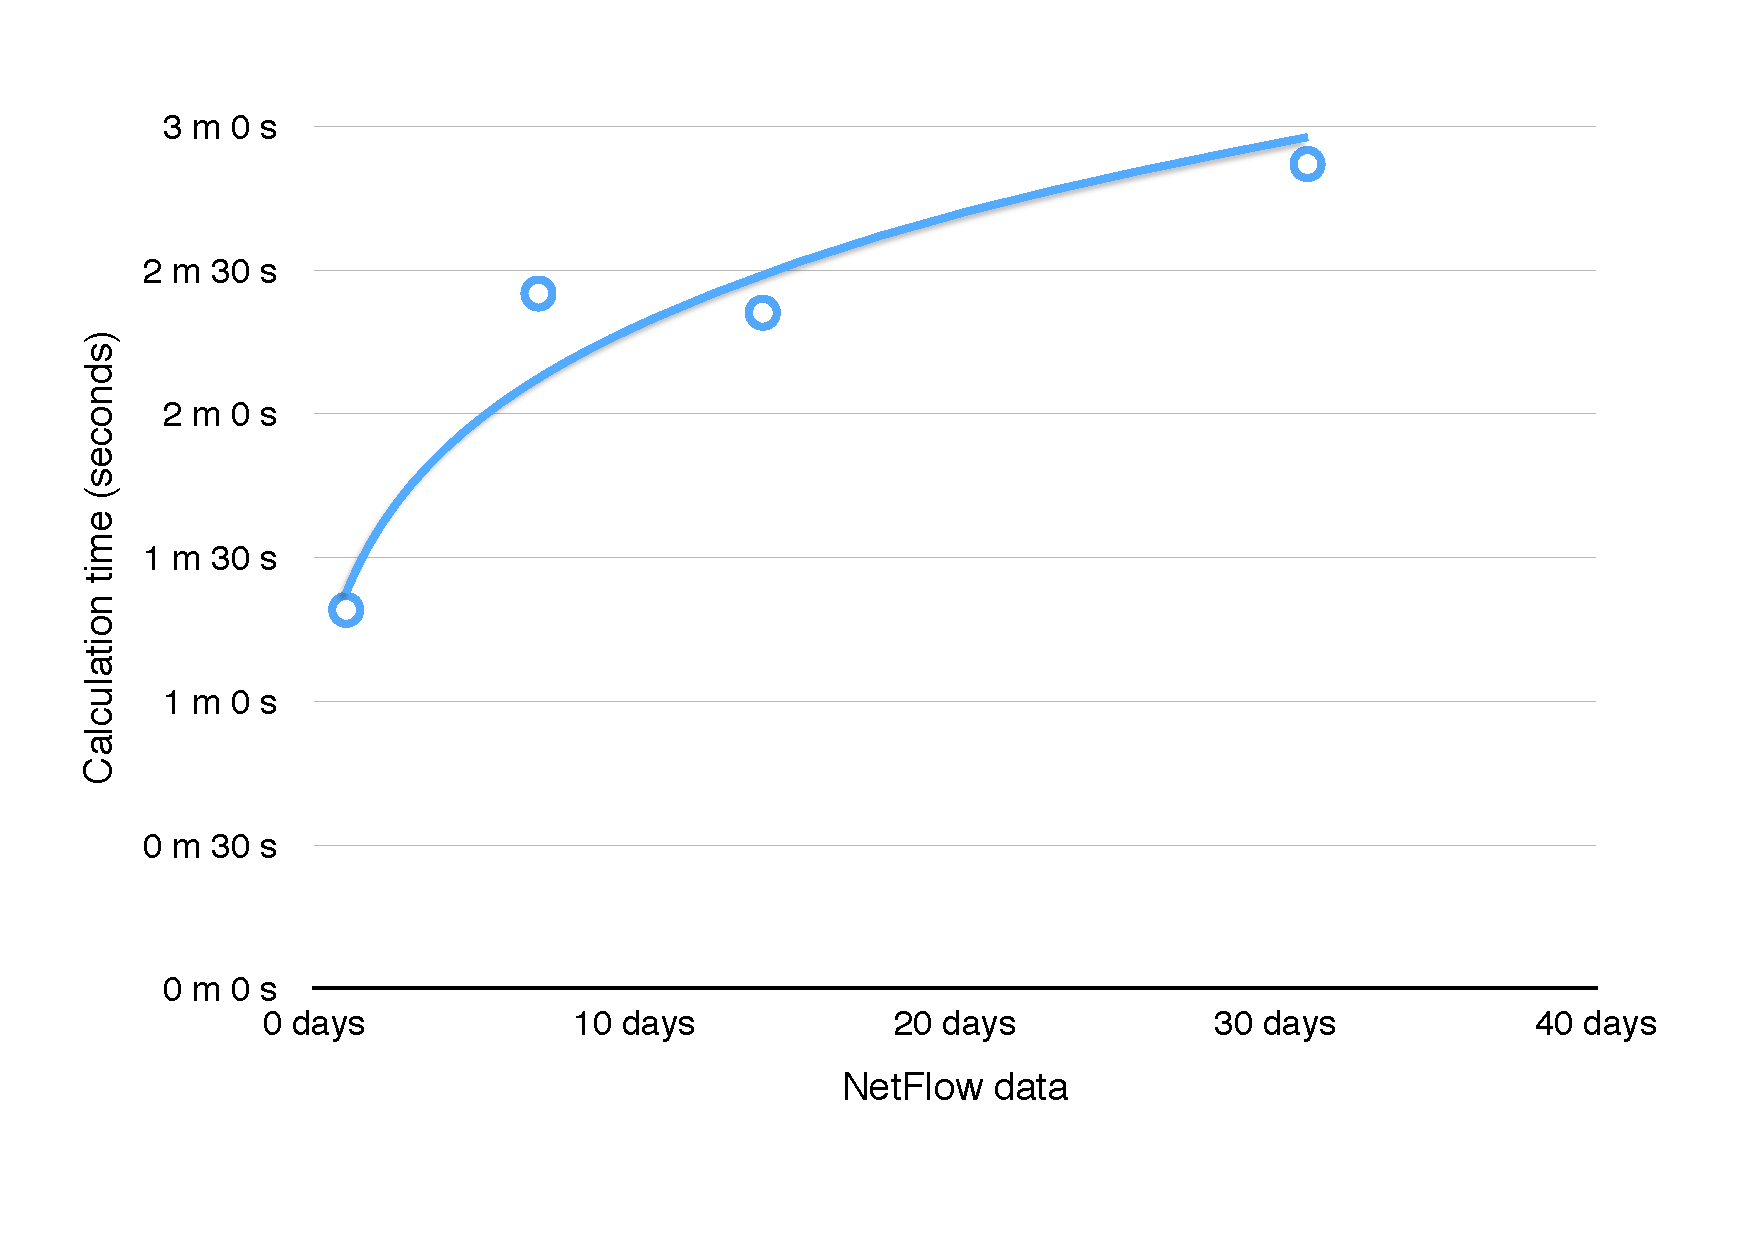
\includegraphics[width=.75\textwidth]{performance}
\end{figure}


\section{Comparison to other systems}
Software already exists to handle NetFlow logs.
The goal of most of this software is to make NetFlow logs easier readable.
UNINETT currently uses NFSEN\footnote{http://nfsen.sourceforge.net} for analysis of NetFlow information.
NFSEN provides a web interface from which the NetFlow log can easily be accessed as text or aggregrated plot (figure~\ref{fig:details-graphs}).
The aggregated data from NFSEN can be generated using MapReduce~\cite{Morken352472}.

\begin{figure}[h!]
	\caption{Screenshot of NFSEN (http://nfsen.sourceforge.net/details-graphs.png)}
	\label{fig:details-graphs}
	\centering
		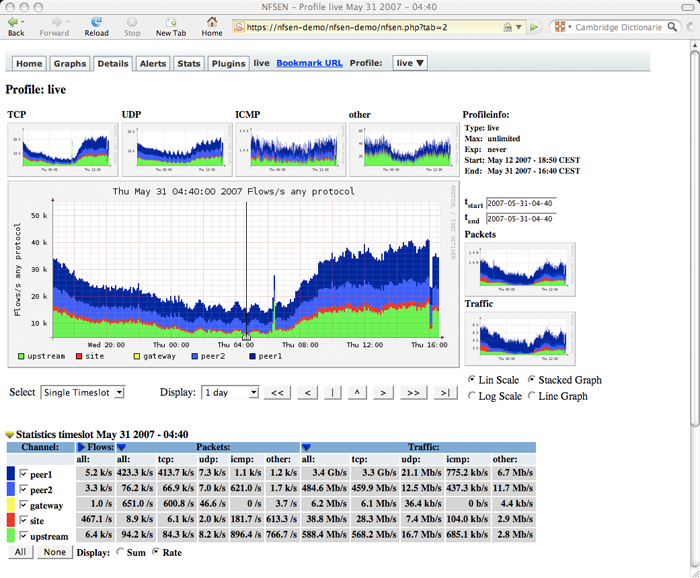
\includegraphics[width=1\textwidth]{details-graphs}
\end{figure}

SpreadRank, as implemented in this thesis, does not provide any database storage, plot generation or user interfaces.
The plots shown in this thesis were created using modeling tools and spreadsheet software.
SpreadRank, instead, aggregates flows in a more recursive way, which gives additional metrics about end-hosts.
These metrics would be useful to integrate in NFSEN, but NFSEN in its current form does not support plugins.
Software similar to NFSEN is FlowViewer\footnote{http://sourceforge.net/projects/flowviewer/} and SiLK~\footnote{https://tools.netsa.cert.org/silk/}.

